\chapter{Dynamic reconfigurable configuration method}  \label{chap:study}
%Experiments on Localization Reliability and Improvement

%This chapter is dedicated to the proposed system which is capable of 

\section{Methodological approach} \label{sec:config-perf}

- tenho sistema que estima os MSE, erro de azimute e elevação, para certas configuração consegue-se perceber padroes nos erros (e.g. erro aumenta com afastamento da source -> ao longe variações pequenas de angulo podem indicar deslocação da estimação grande )
\\
- de entre 8 hidrofones, escolher sempre 3 (+1 no nariz) que minimizam o erro de estimação
\\
- Configurações com vista direta: seccionar campo de visão para cada hidrofone
\\
- aumenta o ângulo de visão para posições no espaço (literature review de valores tipicos)

\section{Systematic analysis of geometric configurations performance} \label{sec:config-perf}

One of the aspects that can be studied to improve the localization estimation is analyzing the best sensor configuration that could be used for a certain scenario. Therefore, it was used the Crámer-Rao lower bound method to do a systematic study on the performance of several hydrophone configurations to be applied in many situations. The study serves as decision method for sensor configurations both applied in an AUV or in a situation without a vehicle. 

The fundamental thought process and mathematical notation used in \ref{sec:cramer} are applied in the study that will be explained next.

\subsection{Analytic Approach}  

Following the logical approach for the process, there are three essential steps that can be differentiated:

\begin{enumerate}
	
	\item Formulate the observations vector
	\item Calculate the Fisher Information Matrix (FIM)
	\item Calculate the determinant of FIM and draw conclusions
	
\end{enumerate}

In this thesis, the number of used hydrophones per estimation is four, so all calculations will be presented for this specific case.

Firstly, the observations vector is formulated based on an initial time of arrival $t_0$, which is given by a synchrony mechanism integrated in the global communication system, and the time-of-arrival based on the vectors that connect the hydrophone positions, $r_i$, to the considered source, $s_t$. For a more realistic approach, it is also considered an added noise component that can be approximated to to a Gaussian distribution $n_i \sim \mathcal{N}(\mu,\,\sigma^{2})$. 

The four observations vector are then formulated as expressed in \ref{eq:obs-my}.

\begin{eqnarray}
t_1 = t_0 + \frac{s_t - r_1}{c} + n_i \\
t_2 = t_0 + \frac{s_t - r_2}{c} + n_i \\
t_3 = t_0 + \frac{s_t - r_3}{c} + n_i \\
t_4 = t_0 + \frac{s_t - r_4}{c} + n_i \\
\label{eq:obs-my}
\end{eqnarray}

Then, addressing the second step, all conditions are set to calculate the FIM,  $I(d) \in \mathbb{R}^{3x3}$. In order to do so, if it is considered d$_{i}$ = $|| s_{t} - r_{i} ||$ as the distance between each sensor and the source, the gradient of the observations vector can be expressed as shown in \ref{eq:grad_fisher}.

\begin{eqnarray}
\nabla_{d}t(d) = \frac{1}{c} 
\begin{bmatrix}
\frac{d_1^T}{||d_1||} \\ 
\addlinespace
\frac{d_2^T}{||d_2||} \\
\vdots \\
\addlinespace
\frac{d_N^T}{||d_N||}
\end{bmatrix}
\label{eq:grad_fisher}
\end{eqnarray}

Additionally, the added noise component which is introduces to the calculations is present in the covariance matrix used in the FIM equation, which is represented as in \ref{eq:covariance}.

\begin{eqnarray}
& \Sigma = 
\begin{bmatrix}
\sigma_1^2 & 0 & 0 & 0 \\
0 & \sigma_2^2 & 0 & 0 \\
0 & 0  & \sigma_3^2  & 0 \\
0 & 0 & 0 & \sigma_4^2 
\end{bmatrix}
\label{eq:covariance}
\end{eqnarray}

Overall, the conditions to obtain the FIM matrix are established and, after some mathematical formulation, it is expressed as \ref{eq:final-fisher}. This expression can be validated by a similar study made on TOA based optimal positioning \cite{cramer-bruno}.

\begin{eqnarray}
I(d) = \frac{1}{c^2} 
\begin{bmatrix}
\sum_{n=1}^{N} \frac{d_i d_i^T}{||d_i||^2} \frac{1}{\sigma_i^2}\\
\end{bmatrix}
\label{eq:final-fisher}
\end{eqnarray}

The final step is to calculate the determinant and find its relation to the volume of the \textit{uncertainty ellipsoid}. As mentioned before, in \ref{sec:cramer}, the determinant of the Fisher Information matrix gives a deterministic value that represents the quantity of information that we can obtain and, therefore, the objective is to maximize it, by respecting the condition $argmax \; det(I(d))$, and consequently minimizing the volume of the ellipsoid. 

\subsubsection{Uncertainty Sphere}

Firstly, it is necessary to choose a set of hydrophone configurations to be tested by the developed simulation environment. Therefore, considering the geometry of an AUV it was formulated a matrix containing nine hydrophones, from which are chosen four at a time to compose the configuration. Matrix \ref{tab:config-9h} represents positions of the the nine hydrophones, where each column expresses the coordinates of each hydrophone, $r_i$, where the value of $x_i$ is in the first row, the value of $y_i$ in the second row and the value of $z_i$ in the third row. Since the configuration has to be three dimensional, it is considered that the hydrophone $r_1$, in the first column, always integrates the configuration since it is the only one in a different plan.

\begin{table}[!htbp] %use H to adjust
	\begin{center}
		\begin{tabular}{|c| c c c c c c c c c|}
			\hline
			
			& r1 & r2 & r3 & r4	& r5 & r6 & r7 & r8	& r9 \\ \hline 
			\multirow{1}{0.5em}{x} 
			& q & 0 & 0 & 0 & 0 & 0 & 0 & 0 & 0\\
			\hline 
			\multirow{1}{0.5em}{y} 
			& 0 & 0 & 0 & w & -w & e & e & -e & -e\\
			\hline 
			\multirow{1}{0.5em}{z} 
			& 0 & w & -w & 0 & 0 & e & -e & e & -e \\
			\hline 
		\end{tabular}
		\caption{Hydrophone geometric positions}
		\label{tab:config-9h}
	\end{center}
\end{table}

In order to evaluate the obtained determinant values, a way to give physical meaning to this result is to analyze it through the uncertainty volume. However, in an initial approach the ellipsoid was not considered and instead an uncertainty sphere was analyzed. The radius of the uncertainty sphere, $us$, is expressed as \ref{eq:det-sphere}, which translates the three ellipsoid axis into a single mean radius that originates a figure of the same volume.

\begin{eqnarray}
& u_{sphere}(d) = \sqrt[2]{\sqrt[3]{det(I(d)^{-1})}}
\label{eq:det-sphere}
\end{eqnarray}

By doing this, we know are looking to find the $argmin ur(d)$ which indicates that the error that originates that uncertainty radius is minimal.

\subsubsection{Uncertainty Ellipsoid}

- eigenvalues give the length of each axis of ellipsoid

\begin{eqnarray}
& u_{ellipsoid}(d) = \sqrt[2]{eig(I(d)^{-1})}
\label{eq:det-ellip}
\end{eqnarray}


\subsection{Simulation Results}

All the concepts and notions before mentioned were applied in a simulated series of scenarios, where it is attempted to take conclusions about optimal positioning of the sensors for performance improvement. As such, the conditions of the simulation as well as the results of the study are hereinafter explained.

As mentioned before, the key to evaluate the performance when adopting this method is to analyze the determinant of the inverted FIM or, alternatively, the matrix's eigenvalues.

%\begin{figure}[!htbp]
%	\centering
%	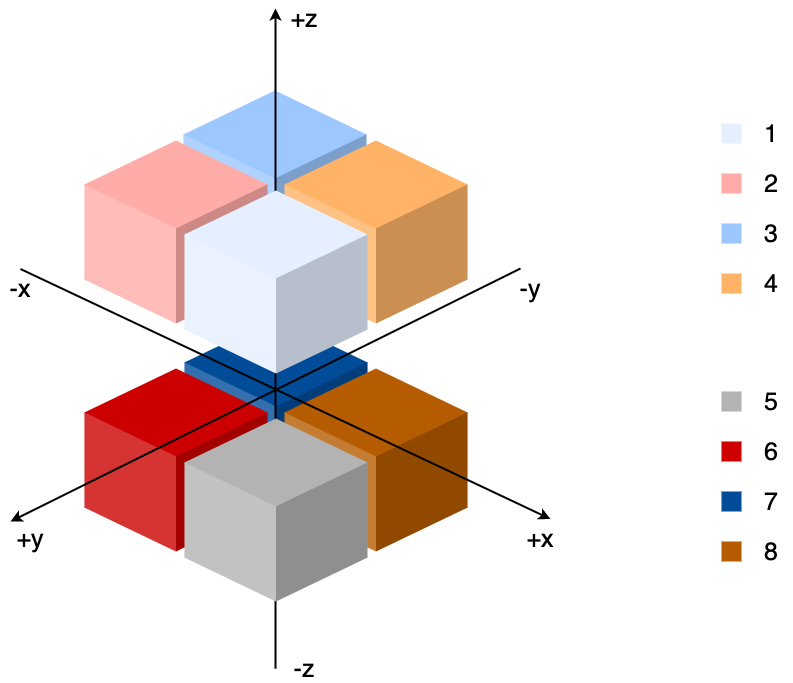
\includegraphics[width=0.7\textwidth]{figures/octant}
%	\caption{Octant discrimination in 3D space}
%	\label{fig:octant}
%\end{figure}



... Layout some results ... 
\\
\\
Ideias:
\\
1-----
\\
- tabela que para cada posição de 4 hidrofones, indica:
\\
- raio de incerteza maximo e posição no espaço onde ocorreu
\\
-raio de incerteza minimo e posição no espaço onde ocorreu
\\
- desvio padrao de todos os pontos no espaço
\\
- uncertainty ellipsoid 
\\
\\
2-----
\\
plot do raio de incerteza para todas as posições no espaço de uma certa configuração

\subsubsection{Conclusions}